\ifdefined \buildingFullOPALManual \else


%\ifx \@buildingFullOPALManual \@empty
%\else

%\documentclass[12pt,a4paper]{report}
\documentclass[a4paper]{book}

%% does not work in Latex2Html mode
%\usepackage{hyperref}

\usepackage[T1]{fontenc}
\usepackage{url}
\usepackage{html}
\usepackage{epic}
\usepackage{eepic}
\usepackage{makeidx}
\usepackage{array}
\usepackage{times}
\usepackage{amsmath}
\usepackage{amsxtra}
\usepackage{bm}
\usepackage[thin,thinp,thinc]{esdiff}
\usepackage{graphicx}
\usepackage{dingbat}
\usepackage{color}
\usepackage{subfig}
\usepackage{boxedminipage}
\usepackage{alltt}
\usepackage{nicefrac}
\usepackage{calc}
%\usepackage{pdfdraftcopy}             % Draft
\usepackage{tikz}
\usetikzlibrary{
  er,3d,calc,fadings,trees,positioning,arrows,chains,decorations.pathreplacing,
  decorations.pathmorphing,shapes,shapes.symbols,shapes.arrows,matrix,through,decorations.text
}

\tikzset{
  >=stealth',
  punktchain/.style={rectangle,rounded corners, draw=black, very thick,text width=10em,
                     minimum height=3em, text centered, on chain},
  line/.style={draw, thick, <-},
  element/.style={tape,top color=white,bottom color=blue!50!black!60!,minimum width=8em,
                  draw=blue!40!black!90, very thick,text width=10em, minimum height=3.5em,
                  text centered, on chain},
  every join/.style={->, thick,shorten >=1pt},
  tuborg/.style={decorate},
  tubnode/.style={midway, right=2pt}
}

\tikzstyle{material}=[draw, fill=blue!20, text width=16.0em, text centered, minimum height=1.5em]
\tikzstyle{diagramstep} = [material, text width=20em, minimum width=10em, minimum height=3em, rounded corners]
\tikzstyle{line} = [draw, thick, color=black!50, -latex']

\usepackage{booktabs}
\usepackage{xspace}
\usepackage{xstring}

\usepackage{fancyvrb}
\usepackage{rotating}
\usepackage{float}

\usepackage{tabularx}
\usepackage{longtable}
\setcounter{LTchunksize}{3}

\usepackage[section]{placeins}
\usepackage{MnSymbol}
\usepackage{microtype}
\usepackage{setspace}
\usepackage{dcolumn}

\usepackage[vmargin={3.0cm,3.0cm},
            hmargin={2.0cm,3.0cm}]{geometry}

\usepackage{upgreek}
\usepackage[binary-units=true]{siunitx}
\sisetup{exponent-product = \cdot,math-ohm=\Upomega,text-ohm=\ensuremath{\Upomega}}
\DeclareSIUnit{\clight}{c}
\DeclareSIUnit\gauss{Ga}

\usepackage{engord}
\usepackage{wasysym}
\DeclareSIUnit[number-unit-product = \,]{\permill}{\permil}

\usepackage{hyperref}
\hypersetup{
    pdftitle          = The OPAL Framework,
    pdfauthor         = {Andreas Adelmann, Achim Gsell, Valeria Rizzoglio, Christof Metzger-Kraus,
                         Yves Ineichen, Xiaoying Pang, Steve Russell, Chuan Wang, Jianjun Yang,
                         Suzanne Sheehy, Chris Rogers, Daniel Winklehner},
    pdfsubject        = User's Reference Manual,
    pdffitwindow      = true,               % page fit to window when opened
    pdfnewwindow      = true,               % links in new window
    colorlinks        = true,               % false: boxed links; true: colored links
    linkcolor         = black!80!green,     % color of internal links
    citecolor         = black!20!red,       % color of links to bibliography
    urlcolor          = blue,               % color of external links
    breaklinks        = true,
    bookmarksnumbered = true,
    plainpages        = false
}

\usepackage{ifthen}

\newif \iflinuxwindows
\linuxwindowstrue   % set this to true when building the manual on Linux or Windows
\iflinuxwindows
\usepackage{epstopdf}
\fi

\usepackage[backend=biber,
            style=phys,
            biblabel=brackets,
            maxnames=3,
            doi=true,
            isbn=true,
            url=true]{biblatex}
%---- macros ----

\renewcommand{\topfraction}{1.0}
\renewcommand{\bottomfraction}{1.0}
\renewcommand{\textfraction}{0.0}
\renewcommand{\arraystretch}{2.0}
\newenvironment{tex2html_nowrap}{}{}


\newcommand{\Newline}{\hfil \\}


\newsavebox{\ExampleBox}
\newenvironment{example}
 {\VerbatimEnvironment
  \begin{flushleft}
  \begin{lrbox}{\ExampleBox}
    \begin{minipage}{\linewidth}
  \begin{Verbatim}[frame=lines,xleftmargin=0cm,fontsize=\footnotesize,samepage=true]}
 {\end{Verbatim}
  \end{minipage}
  \end{lrbox}
  \mbox{\usebox{\ExampleBox}}
  \end{flushleft}
 }

\newenvironment{longexample}
{\Verbatim[frame=lines,xleftmargin=0mm,fontsize=\footnotesize]}
{\endVerbatim}

%\examplefromfile{filename} reads in a text file and displays it in the document.
\newcommand{\examplefromfile}[1]{
\VerbatimInput[frame=lines,xleftmargin=0mm,fontsize=\footnotesize,label=\texttt{#1}]{#1}}

%for upright d of differentials
\makeatletter
\newcount\my@repeat@count

\newcommand{\myrepeat}[2]{%
  \begingroup
  \my@repeat@count=\z@
  \@whilenum\my@repeat@count<#1\do{#2\advance\my@repeat@count\@ne}%
  \endgroup
}

\newcommand{\differential}[1]{\ifstrempty{#1}{\ES@dop\ES@difint}{\ES@dop^{#1}\ES@difint}}
\newcommand{\pdifferential}[1]{\ifstrempty{#1}{{\partial\,}}{{\partial^{#1}\,}}}

\makeatother

\newcommand{\der}[3][]{\frac{\differential{#1}#2}{\differential{}\ifstrempty{#1}{#3}{#3^#1}}}
\newcommand{\parder}[3][]{\frac{\pdifferential{#1}#2}{\pdifferential{}\ifstrempty{#1}{#3}{#3^#1}}}
\newcommand{\niceder}[3][]{\nicefrac{\differential{#1}#2}{\differential{}\ifstrempty{#1}{#3}{#3^#1}}}
\newcommand{\uglyder}[3][]{{\differential{#1}#2}/{\differential{}\ifstrempty{#1}{#3}{#3^#1}}}
\newcommand{\uglyparder}[3][]{{\pdifferential{#1}#2}/{\pdifferential{}\ifstrempty{#1}{#3}{#3^#1}}}
\newcommand{\dd}[1][]{\; \differential{#1}}
\newcommand{\primed}{^{\prime}}
\newcommand{\dprimed}{^{\prime\prime}}
\newcommand{\nprimed}[1]{^{\myrepeat{#1}{\prime}}}

%Editing Macros
\newcommand{\TODO}[1]{{\color{red}\ifthenelse{\boolean{ShowDebug}}{[TODO: #1]}{}}}



%text in gray box
\newsavebox{\fmbox}
\definecolor{lightgray}{gray}{0.95}
\newenvironment{fmpage}
   {\vspace{-1.0cm}\begin{lrbox}{\fmbox}\begin{minipage}[t]{13.5cm}\vspace{0.1cm}}
   {\vspace{-0.4cm}\end{minipage}\end{lrbox}\begin{center}\fcolorbox{black}{lightgray}{\usebox{\fmbox}}\end{center}}


% Definition new signes
\newcommand{\R}{{\mathbb R}} % real numbers
\newcommand{\Q}{{\mathbb Q}} % rational numbers
\newcommand{\Z}{{\mathbb Z}} % integer numbers
\newcommand{\N}{{\mathbb N}} % natural numbers

\newcommand{\mad}{\textsc{mad}\xspace}
\newcommand{\madnine}{\textsc{mad9}\xspace}
\newcommand{\madninep}{\textsc{mad9p}\xspace}
\newcommand{\madeight}{\textsc{mad8}\xspace}
\newcommand{\classic}{\textsc{classic}\xspace}

\makeatletter
\newcommand{\opal@impl}{\textsc{Opal}}
\newcommand{\opalt@impl}{\textsc{Opal-t}}
\newcommand{\opalcycl@impl}{\textsc{Opal-cycl}}
\newcommand{\opalmap@impl}{\textsc{Opal-map}}
\newcommand{\opalenv@impl}{\textsc{Opal-e}}

\newcommand{\opal}{\opal@impl\xspace}
\newcommand{\opalt}{\opalt@impl\xspace}
\newcommand{\opalcycl}{\opalcycl@impl\xspace}
\newcommand{\opalmap}{\opalmap@impl\xspace}
\newcommand{\opalenv}{\opalenv@impl\xspace}

\newcommand{\noopalt}{\leftthumbsdown \opalt@impl\xspace}
\newcommand{\noopalcycl}{\leftthumbsdown \opalcycl@impl\xspace}
\newcommand{\noopalmap}{\leftthumbsdown \opalmap@impl\xspace}
\newcommand{\noopalenv}{\leftthumbsdown \opalenv@impl\xspace}
\makeatother

\newcommand{\impactt}{\textsc{Impact-t}\xspace}
\newcommand{\partroot}{\textsc{H5root}}


\newcommand{\latermore}{More details will be given in Version 1.6.0}


\newcommand{\lieop}[1]{{:}{#1}{:}}

\newcommand{\rms}[1]{\overset{\sim}{#1}}

\newcommand{\sprod}{\cdot}
\newcommand{\vprod}{\times}
\newcommand{\matr}[1]{\mathcal{#1}}
\renewcommand{\vec}[1]{{\bm{#1}}}
\newcommand{\transpose}[1]{#1^\intercal}
\renewcommand{\epsilon}{\varepsilon}

\newcommand{\keyword}[2][]{\ifstrempty{#1}{\texttt{\expandafter\MakeUppercase\expandafter{#2}}}{\hyperref[#1]{\texttt{\expandafter\MakeUppercase\expandafter{#2}}}}}
\newcommand{\tabline}[3][]{\keyword[#1]{#2}& #3 \\}
\newcommand{\tabheadcell}[1]{{\bfseries #1}}

\newcommand*\kdescriptionlabel[1]{\hspace\labelsep
                                \normalfont\keyword{#1}\index{#1}}
\makeatletter
\newenvironment{kdescription}
               {\list{}{\labelwidth\z@ \itemindent-\leftmargin
                        \let\makelabel\kdescriptionlabel}}
               {\endlist}
\makeatother

\ExplSyntaxOn
\NewDocumentCommand{\tabhead}{ m }
 {
  \seq_set_split:Nnn \l_tmpa_seq { & } { #1 }
  \bfseries \seq_use:Nn \l_tmpa_seq { & \bfseries } \\
 }

\NewDocumentCommand \multrefImpl { O{ } m m m } {
  \ifnumgreater{\clist_count:n {#4}}{1}{
    \seq_set_from_clist:Nn \l_tmpa_seq { #4 }

    \seq_set_map:NNn \l_tmpb_seq \l_tmpa_seq { \exp_not:n { \ref{#3:##1} } }
    \ifstrempty{#1}{#2s}{#1}~\seq_use:Nnnn \l_tmpb_seq {\ and\ } {,\ } {,\ and\ }
  }{
    #2~\ref{#3:#4}
  }
}

\NewDocumentCommand \multeqnrefImpl { m } {
  \ifnumgreater{\clist_count:n {#1}}{1}{
    \seq_set_from_clist:Nn \l_tmpa_seq { #1 }

    \seq_set_map:NNn \l_tmpb_seq \l_tmpa_seq { \exp_not:n { \eqref{eq:##1} } }
    Equations~\seq_use:Nnnn \l_tmpb_seq {\ and\ } {,\ } {,\ and\ }
  }{
    Equation~\eqref{eq:#1}
  }
}
\ExplSyntaxOff


%Abbreviations for Equations, Figures, and Tables
%\newcommand{\Equation}[1]{Equation~\eqref{#1}}

\newcommand{\bibref}[2]{#1 \cite{bib:#2}}
\newcommand{\figref}[1]{\multrefImpl{Figure}{fig}{#1}}
\newcommand{\chpref}[1]{\multrefImpl{Chapter}{chp}{#1}}
\newcommand{\appref}[1]{\multrefImpl[Appendices]{Appendix}{chp}{#1}}
\newcommand{\secref}[1]{\multrefImpl{Section}{sec}{#1}}
\newcommand{\ssecref}[1]{\multrefImpl{Section}{ssec}{#1}}
\newcommand{\tabref}[1]{\multrefImpl{Table}{tab}{#1}}
\newcommand{\eqnref}[1]{\multeqnrefImpl{#1}}

\newcommand{\seefig}[1]{(see~\figref{#1})}
\newcommand{\seechp}[1]{(see~\chpref{#1})}
\newcommand{\seesec}[1]{(see~\secref{#1})}
\newcommand{\seessec}[1]{(see~\ssecref{#1})}
\newcommand{\seetab}[1]{(see~\tabref{#1})}
\newcommand{\seeeqn}[1]{(see~\eqnref{#1})}

\newcommand{\filename}[1]{\emph{#1}}


% Define distances for bordering
\newcommand{\blockdist}{1.3}
\newcommand{\edgedist}{1.5}
\newcommand{\diagramstep}[2]{node (p#1) [diagramstep] {#2}}


% place chapter title page on odd pages
\let\stdchapter\chapter
\makeatletter
\renewcommand*{\chapter}{\if@openright\cleardoublepage\else\clearpage\fi\stdchapter}

\makeatother

\IfFileExists{./version.tex}{%
  \newcommand{\opalversion}[1]{Version \ifstrempty{#1}{1.9.0}{#1}\xspace}
%
}%
{%
  \newcommand{\opalversion}[1]{\ifstrempty{#1}{current Version}{Version #1}\xspace}%
}
\newboolean{ShowMap}
\setboolean{ShowMap}{false}

\newboolean{ShowEnv}
\setboolean{ShowEnv}{false}

\newboolean{ShowDebug}
\setboolean{ShowDebug}{false}

%----Control Structures
\newboolean{FullOPALManual}
\setboolean{FullOPALManual}{false}


\makeindex


\bibliography{bibliography}
\begin{document}

\fi

\chapter{\opalt}
\label{chp:opalt}
\index{OPAL-t}
\index{PARALLEL-T}
\section{Introduction}
\opalt is a fully three-dimensional program to track in time, relativistic particles taking into account space charge forces, self-consistently in the electrostatic approximation, and short-range longitudinal and transverse wake fields. \opalt is one of the few
codes  that is implemented using a parallel programming paradigm from the ground up. This makes \opalt indispensable for
high statistics simulations of various kinds of existing and new accelerators. It has a comprehensive set of beamline
elements, and furthermore allows arbitrary overlap of their fields, which gives \opalt a capability
to model both the standing wave structure and traveling wave structure. Beside IMPACT-T it is the only code making use of
space charge solvers based on an integrated Green \cite{qiang2005, qiang2006-1,qiang2006-2} function to efficiently and accurately treat beams with
large aspect ratio, and a shifted Green function to efficiently treat image charge effects of a cathode \cite{fubiani2006, qiang2005, qiang2006-1,qiang2006-2}.
For simulations of particles sources i.e. electron guns \opalt uses the technique of  energy binning in the electrostatic space charge calculation to model beams with large
energy spread. In the very near future a parallel Multigrid solver taking into account the exact geometry will be implemented.

\section{Variables in \opalt}
\label{sec:variablesopalt}
\index{OPAL-t!Variables}

\label{sec:opalt:canon}
\index{Canonical Variables}
\index{Variables!Canonical}
\opalt uses the following canonical variables
to describe the motion of particles. The physical units are listed in square brackets.

\begin{description}
\item[X]
  Horizontal position $x$ of a particle relative to the axis of the element [m].

\item[PX]
  $\beta_x\gamma$ Horizontal canonical momentum [1].

\item[Y]
  Horizontal position $y$ of a particle relative to the axis of the element [m].

\item[PY]
  $\beta_y\gamma$ Horizontal canonical momentum [1].

\item[Z]
  Longitudinal position $z$ of a particle in floor co-ordinates [m].

\item[PZ]
 $\beta_z\gamma$ Longitudinal canonical momentum [1].

 \end{description}

The independent variable is  \textbf{t} [s].



\section{Integration of the Equation of Motion}
\opalt integrates the relativistic Lorentz equation
\begin{equation} \diff{\gamma\vec{v}}{t}
 =   \frac{q}{m}[\vec{E}_{ext} + \vec{E}_{sc} + \vec{v} \times (\vec{B}_{ext} + \vec{B}_{sc})]
\end{equation}
where $\gamma$ is the relativistic factor, $q$ is the charge, and $m$ is the rest mass of the particle. $\vec{E}$  and $\vec{B}$ are abbreviations for the electric field $\vec{E}(\vec{x},t)$ and  magnetic field $\vec{B}(\vec{x},t)$. To update the positions and momenta \opalt uses the Boris-Buneman algorithm \cite{langdon}.


\section{Positioning of Elements}
Since \opalversion{2.0} of \opal elements can be placed in space using 3D coordinates \keyword{X}, \keyword{Y}, \keyword{Z}, \keyword{THETA}, \keyword{PHI} and \keyword{PSI}, see \secref{Element:common}. The old notation using \keyword{ELEMEDGE} is still supported. \opalt then computes the position in 3D using \keyword{ELEMDGE}, \keyword{ANGLE} and \keyword{DESIGNENERGY}. It assumes that the trajectory consists of straight lines and segments of circles. Fringe fields are ignored. For cases where these simplifications aren't justifiable the user should use 3D positioning. For a simple switchover \opal writes a file \filename{\_3D.opal} where all elements are placed in 3D.

Beamlines containing guns should be supplemented with the element \keyword[sec:source]{SOURCE}. This allows \opal to distinguish the cases and adjust the initial energy of the reference particle.

Prior to \opalversion{2.0} elements needed only a defined length. The transverse extent was not defined for elements except when combined with 2D or 3D field maps. An aperture had to be designed to give elements a limited extent in transverse direction since elements now can be placed freely in three-dimensional space. See \secref{Element:common} for how to define an aperture.
\section{Coordinate Systems}
\label{sec:CoordinateSystems}
The motion of a charged particle in an accelerator can be described by relativistic Hamilton mechanics.
A particular motion is that of the reference particle, having the central energy and traveling on the
so-called reference trajectory. Motion of a particle close to this fictitious reference particle
can be described by linearized equations for the displacement of the particle under study, relative to the
reference particle. In \opalt, the time $t$ is used as independent variable instead of the path length $s$. The relation between them can be expressed as
\begin{equation}
\frac{\differential{}}{\differential{} t} = \frac{\differential{}}{\differential{}\vec{s}}\frac{\differential{}\vec{s}}{\differential{} t} = \vec{\beta}c\frac{\differential{}}{\differential{}\vec{s}}.
\end{equation}
\subsubsection{Global Cartesian Coordinate System}
We define the global cartesian coordinate system, also known as floor coordinate system with $K$, a point in this coordinate system is denoted by $(X, Y, Z) \in K$.
In \figref{KS1} of the accelerator is uniquely defined by the sequence of physical elements in $K$.
The beam elements are numbered $e_0, \ldots , e_i, \ldots e_n$.
\begin{figure}[!htb]
\begin{center}
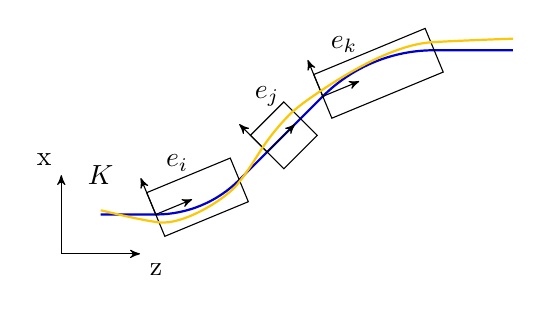
\begin{tikzpicture}
\draw[<->] (0,1cm) |- (1cm, 0);
\node[anchor=north west] at (1cm,0) {z};
\node[anchor=south east] at (0,1cm) {x};
\node at (0.5cm, 1cm) {$K$};
\draw[color=blue!80!black,thick] (0.5cm,0.5cm) -- (1.2cm,0.5cm) arc (270:315:1.5cm) -- ++(45:1.5cm) arc (135:90:2cm) --++(0:1cm);
\begin{scope}[cm={0.9239,0.3827,-0.3827,0.9239,(1.2cm,0.5cm)}]
    \draw (0,-0.3cm) rectangle (1.148cm,0.3cm);
    \draw[<->] (0.5cm,0)-|(0,0.5cm);
    \node at (0.5cm, 0.5cm) {$e_i$};
\end{scope}
\begin{scope}[cm={0.7071,0.7071,-0.7071,0.7071,(2.6142,1.2929)}]
    \draw (0,-0.3cm) rectangle (0.6cm,0.3cm);
    \draw[<->] (0.5cm,0)-|(0,0.5cm);
    \node at (0.5cm, 0.5cm) {$e_j$};
\end{scope}
\begin{scope}[cm={0.9239,0.3827,-0.3827,0.9239,(3.3213cm,2cm)}]
    \draw (0,-0.3cm) rectangle (1.5307cm,0.3cm);
    \draw[<->] (0.5cm,0)-|(0,0.5cm);
    \node at (0.5cm, 0.5cm) {$e_k$};
\end{scope}
\path[cm={2.849,0,0,2.849,(-8.4571,25.7235)},draw=yellow!80!red,line width=0.800pt]
  (3.144,-8.835) .. controls
  (3.144,-8.833) and (3.286,-8.872) .. (3.398,-8.888) .. controls
  (3.511,-8.905) and (3.705,-8.782) .. (3.755,-8.717) .. controls
  (3.801,-8.659) and (3.820,-8.626) .. (3.867,-8.553) .. controls
  (3.896,-8.509) and (3.955,-8.436) .. (3.999,-8.396) .. controls
  (4.044,-8.357) and (4.066,-8.343) .. (4.127,-8.301) .. controls
  (4.190,-8.260) and (4.427,-8.100) .. (4.615,-8.086) .. controls
  (4.689,-8.081) and (4.906,-8.072) .. (4.983,-8.070);
\end{tikzpicture}
  \caption{Illustration of local and global coordinates.}
  \label{fig:KS1}
\end{center}
\end{figure}

\subsubsection{Local Cartesian Coordinate System}
A local coordinate system $K'_i$ is attached to each element $e_i$. This is simply a frame in which $(0,0,0)$ is at the entrance of  each element. For an illustration see \figref{KS1}. The local reference system $(x, y, z) \in K'_n$
may thus be referred to a global Cartesian coordinate system $(X, Y, Z) \in K$.

The local coordinates $(x_i, y_i, z_i)$ at element $e_i$ with respect to the global coordinates $(X, Y, Z)$ are defined by three displacements $(X_i, Y_i, Z_i)$ and three angles $(\Theta_i, \Phi_i, \Psi_i)$.

$\Psi$ is the roll angle about the global $Z$-axis. $\Phi$ is the pitch angle about the global $Y$-axis. Lastly, $\Theta$ is the yaw angle about the global $X$-axis. All three angles form right-handed screws with their corresponding axes. The angles ($\Theta,\Phi,\Psi$) are the  Tait-Bryan angles \cite{bib:tait-bryan}.

The displacement is described by a vector $\vec{v}$
and the orientation by a unitary matrix $\matr{W}$.
The column vectors of $\matr{W}$ are unit vectors spanning
the local coordinate axes in the order $(x, y, z)$.
$\vec{v}$ and $\matr{W}$ have the values:
\begin{equation}
\vec{v} =\left(\begin{array}{c}
    X \\
    Y \\
    Z
  \end{array}\right),
\qquad
\matr{W}=\matr{S}\matr{T}\matr{U}
\end{equation}
where
\begin{equation}
\matr{S}=\left(\begin{array}{ccc}
    \cos\Theta &  0 &  \sin\Theta \\
    0         &  1 &   0 \\
    -\sin\Theta &  0 &  \cos\Theta
  \end{array}\right),
\quad
\matr{T}=\left(\begin{array}{ccc}
    1 &  0        &  0 \\
    0 &  \cos\Phi &  \sin\Phi \\
    0 & -\sin\Phi &  \cos\Phi
  \end{array}\right),
\end{equation}
\begin{equation}
\matr{U}=\left(\begin{array}{ccc}
    \cos\Psi & -\sin\Psi &  0 \\
    \sin\Psi &  \cos\Psi &  0 \\
    0        &  0        &  1
  \end{array}\right).
\end{equation}


We take the vector $\vec{r}_i$ to be the displacement and the matrix
$\matr{S}_i$ to be the rotation of the local reference system
at the exit of the element $i$ with respect to the entrance
of that element.

Denoting with $i$ a beam line element,
one can compute $\vec{v}_i$ and $\matr{W}_i$
by the recurrence relations
\begin{equation} \label{eq:surv}
\vec{v}_i = \matr{W}_{i-1}\vec{r}_i + \vec{v}_{i-1}, \qquad
\matr{W}_i = \matr{W}_{i-1}\matr{S}_i,
\end{equation}
where $\vec{v}_0$ corresponds to the origin of the \keyword{LINE} and $\matr{W}_0$ to its orientation. In \opalt they can be defined using either \keyword{X}, \keyword{Y}, \keyword{Z}, \keyword{THETA}, \keyword{PHI} and \keyword{PSI} or \keyword{ORIGIN} and \keyword{ORIENTATION}, see \secref{line:simple}.

\subsubsection{Space Charge Coordinate System}
In order to calculate space charge in the electrostatic approximation, we introduce a co-moving coordinate system $K_{\text{sc}}$, in which the origin coincides with the mean position of the particles and the mean momentum is parallel to the z-axis.


\subsubsection{Curvilinear Coordinate System}
In order to compute statistics of the particle ensemble, $K_s$ is introduced.
The accompanying tripod (Dreibein) of the reference orbit spans
a local curvilinear right handed system $(x,y,s)$.
The local $s$-axis is the tangent to the reference orbit.
The two other axes are perpendicular to the reference orbit and
are labelled~$x$ (in the bend plane)
and~$y$ (perpendicular to the bend plane).
\begin{figure}[!htb]
\begin{center}
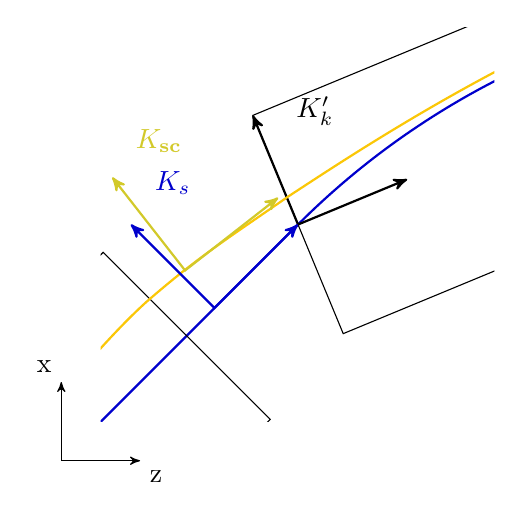
\begin{tikzpicture}
\draw[<->] (0,1cm) |- (1cm, 0);
\node[anchor=north west] at (1cm,0) {z};
\node[anchor=south east] at (0,1cm) {x};
\begin{scope}[cm={5,0,0,5,(-13.6,-7)}]
\begin{scope}
\clip (2.82,1.5) rectangle (3.82,2.5);
\draw[color=blue!80!black,thick] (0.5cm,0.5cm) -- (1.2cm,0.5cm) arc (270:315:1.5cm) -- ++(45:1.5cm) arc (135:90:2cm) --++(0:1cm);
\begin{scope}[cm={0.9239,0.3827,-0.3827,0.9239,(1.2cm,0.5cm)}]
    \draw (0,-0.3cm) rectangle (1.148cm,0.3cm);
%    \draw[<->] (0.5cm,0)-|(0,0.5cm);
    \node at (0.5cm, 0.5cm) {$e_i$};
\end{scope}
\begin{scope}[cm={0.7071,0.7071,-0.7071,0.7071,(2.6142,1.2929)}]
    \draw (0,-0.3cm) rectangle (0.6cm,0.3cm);
%    \draw[<->] (0.5cm,0)-|(0,0.5cm);
    \node at (0.5cm, 0.5cm) {$e_j$};
\end{scope}
\begin{scope}[cm={0.9239,0.3827,-0.3827,0.9239,(3.3213cm,2cm)}]
    \draw (0,-0.3cm) rectangle (1.5307cm,0.3cm);
    \draw[<->,thick] (0.3cm,0)-|(0,0.3cm);
    \node at (0.15cm, 0.25cm) {$K\primed_k$};
\end{scope}
\path[cm={2.849,0,0,2.849,(-8.4571,25.7235)},draw=yellow!80!red,line width=0.800pt]
  (3.144,-8.835) .. controls
  (3.144,-8.833) and (3.286,-8.872) .. (3.398,-8.888) .. controls
  (3.511,-8.905) and (3.705,-8.782) .. (3.755,-8.717) .. controls
  (3.801,-8.659) and (3.820,-8.626) .. (3.867,-8.553) .. controls
  (3.896,-8.509) and (3.955,-8.436) .. (3.999,-8.396) .. controls
  (4.044,-8.357) and (4.066,-8.343) .. (4.127,-8.301) .. controls
  (4.190,-8.260) and (4.427,-8.100) .. (4.615,-8.086) .. controls
  (4.689,-8.081) and (4.906,-8.072) .. (4.983,-8.070);
\end{scope}
\begin{scope}[cm={0.7071,0.7071,-0.7071,0.7071,(3.109,1.788)}]
\draw[<->,blue!80!black,thick] (0.3,0.0) -| (0.0,0.3);
\node[blue!80!black] at (0.15cm, 0.3cm) {$K_s$};
\end{scope}
\begin{scope}[cm={0.788,0.616,-0.616,0.788,(3.109,1.788)}]
\draw[<->,yellow!80!black,thick] (0.3,0.121) -| (0.0,0.421);
\node[yellow!80!black] at (0.15cm, 0.421cm) {\textbf{$K_{\text{sc}}$}};
\end{scope}
\end{scope}
\end{tikzpicture}
  \caption{Illustration of $K_\text{sc}$ and $K_s$}
  \label{fig:KS2}
\end{center}
\end{figure}
Both coordinate systems are described in \figref{KS2}.

\subsection{Design or Reference Orbit}
The reference orbit consists of a series of straight sections and circular arcs and is {\bf computed} by the Orbit Threader i.e. deduced from the element placement in the floor coordinate system.

\subsection{Compatibility Mode}
To facilitate the change for users we will provide a compatibility mode. The idea is that the user does not have to change the input file. Instead \opalt will compute the positions of the elements. For this it uses the bend angle and chord length of the dipoles and the position of the elements along the trajectory. The user can choose whether effects due to fringe fields are considered when computing the path length of dipoles or not. The option to toggle \opalt's behavior is called \keyword{IDEALIZED}. \opalt assumes per default that provided \keyword{ELEMEDGE} for elements downstream of a dipole are computed without any effects due to fringe fields.

Elements that overlap with the fields of a dipole have to be handled separately by the user to position them in 3D.

We split the positioning of the elements into two steps. In a first step we compute the positions of the dipoles. Here we assume that their fields don't overlap. In a second step we can then compute the positions and orientations of all other elements.

The accuracy of this method is good for all elements except for those that overlap with the field of a dipole.

\subsection{Orbit Threader and Autophasing}
\label{sec:orbitthreader}
The \texttt{OrbitThreader} integrates a design particle through the lattice and setups up a multi map structure (\texttt{IndexMap}). Furthermore when the reference particle hits an rf-structure for the first time then it auto-phases the rf-structure, see \appref{autophasing}. The multi map structure speeds up the search for elements that influence the particles at a given position in 3D space by minimizing the looping over elements when integrating an ensemble of particles. For each time step, \texttt{IndexMap} returns a set of elements $\mathcal{S}_{\text{e}} \subset {e_0 \ldots e_n}$ in case of the example given in \figref{KS1}. An implicit drift is modelled as an empty set $\emptyset$.

\subsection{Flow Diagram of \opalt}
\begin{figure}[!htb]
  \centering
 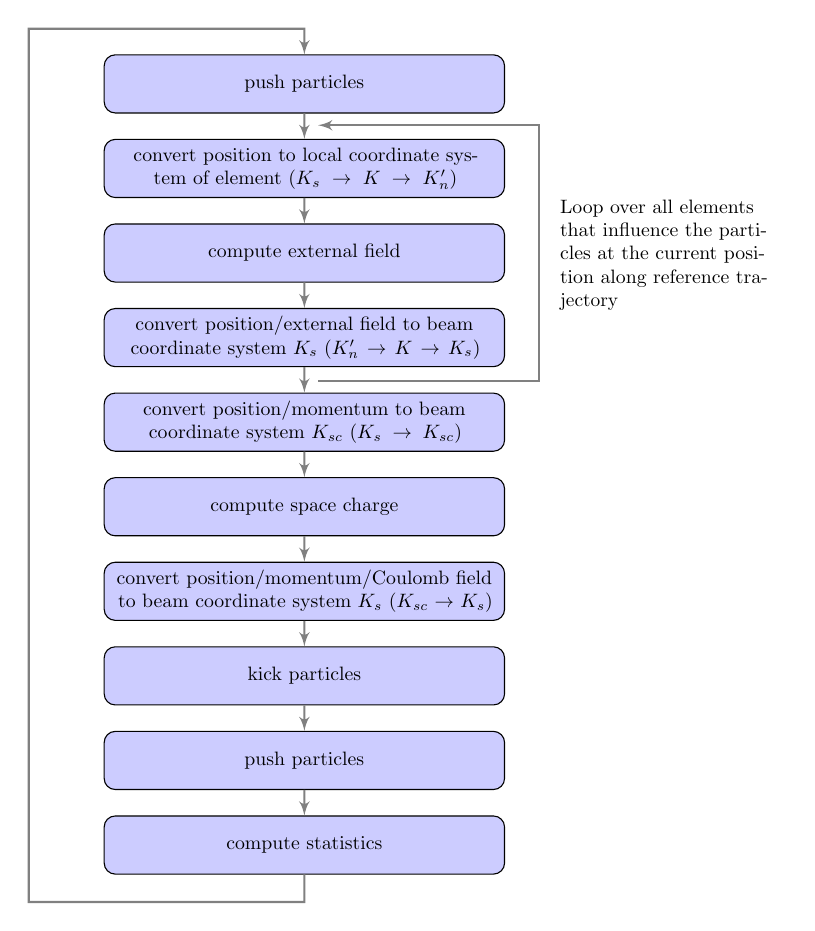
\begin{tikzpicture}[scale=0.7,transform shape]

  % Draw diagram elements
  \path \diagramstep {1}{push particles};
  \path (p1.south)+(0.0,-1.0) \diagramstep{2}{convert position to local coordinate system of element ($K_s \rightarrow K \rightarrow K'_n$)};
  \path (p2.south)+(0.0,-1.0) \diagramstep{3}{compute external field};
  \path (p3.south)+(0.0,-1.0) \diagramstep{4}{convert position/external field to beam coordinate system $K_s$ ($K'_n \rightarrow K \rightarrow K_s$)};
  \path (p4.south)+(0.0,-1.0) \diagramstep{5}{convert position/momentum to beam coordinate system $K_{sc}$ ($K_s \rightarrow K_{sc}$)};
  \path (p5.south)+(0.0,-1.0) \diagramstep{6}{compute space charge};
  \path (p6.south)+(0.0,-1.0) \diagramstep{7}{convert position/momentum/Coulomb field to beam coordinate system $K_s$ ($K_{sc} \rightarrow K_s$)};
  \path (p7.south)+(0.0,-1.0) \diagramstep{8}{kick particles};
  \path (p8.south)+(0.0,-1.0) \diagramstep{9}{push particles};
  \path (p9.south)+(0.0,-1.0) \diagramstep{11}{compute statistics};

  % Draw arrows between elements
  \path [line] (p1.south) -- node [above] {} (p2);
  \path [line] (p2.south) -- node [above] {} (p3);
  \path [line] (p3.south) -- node [above] {} (p4);
  \path [line] (p4.south) -- node [above] {} (p5);
  \path [line] (p5.south) -- node [above] {} (p6);
  \path [line] (p6.south) -- node [above] {} (p7);
  \path [line] (p7.south) -- node [above] {} (p8);
  \path [line] (p8.south) -- node [above] {} (p9);
  \path [line] (p9.south) -- node [above] {} (p11);
  \path [line] (p11.south) -- +(0.0, -0.5) -- +(-5.0,-0.5) |- (0.0, 1.0) -- (p1);

  \node[anchor=center,text width=4cm] at ($(p4.east)+(3.0,1.5)$) (nodeA) {Loop over all elements that influence the particles at the current position along reference trajectory};

  \path [line] ($(p4.south)+(0.25,-0.25)$) -- +(4.0, -0.0) |- ($(p2.north)+(0.25,0.25)$);

%  \path [line,
%                  postaction={decorate},
%                  decoration={text along path,
%                  text= for all elements,
%                  text align={left indent={0.7\dimexpr\pgfdecoratedpathlength\relax}}
%                  }
%  ] (p4.west) -- +(-3.0, -0.0) -- +(-3.0, 3.0) -- (p2.west);
\end{tikzpicture}
  \caption{Schematic workflow of \opalt's execute method.}
  \label{fig:OPALTSchemeSimple}
\end{figure}
A regular time step in \opalt is sketched in \figref{OPALTSchemeSimple}. In order to compute the coordinate system transformation from the reference coordinate system $K_s$ to the local coordinate systems $K'_n$ we join the transformation from floor coordinate system $K$ to $K'_n$ to the transformation from $K_s$ to $K$. All computations of rotations which are involved in the computation of coordinate system transformations are performed using quaternions. The resulting quaternions are then converted to the appropriate matrix representation before applying the rotation operation onto the particle positions and momenta.

As can be seen from \figref{OPALTSchemeSimple} the integration of the trajectories of the particles are integrated and the computation of the statistics of the six-dimensional phase space are performed in the reference coordinate system.

\section{Output}
In addition to the progress report that \opalt writes to the standard output (stdout) it also writes different files for various purposes.
\subsubsection*{\filename{\textless input\_file\_name \textgreater.stat}}
This file is used to log the statistical properties of the bunch in the ASCII variant of the SDDS format \cite{bib:borland1995}. It can be viewed with the SDDS Tools \cite{bib:borland2016} or GNUPLOT. The frequency with which the statistics are computed and written to file can be controlled With the option \keyword{STATDUMPFREQ}. The information that is stored are found in the following table.
\begin{center}
\begin{longtable}{p{1.2cm}p{1.9cm}p{1.3cm}p{9.5cm}}
\caption{Information stored in the file \filename{\textless input\_file\_name \textgreater.stat}}\\
\hline
\tabhead{Column Nr. & Name & Units & Meaning}
\hline
\endfirsthead
\hline
\multicolumn{4}{c}{{\bfseries \tablename\ \thetable{} -- continued}}\\
\tabhead{Column Nr. & Name & Units & Meaning}
\hline
\endhead
%\hline
\multicolumn{4}{r}{{Continued on next page...}}\\
\hline
\endfoot
\hline
\endlastfoot
1 & t & \si{\nano\second} & Time\\
2 & s & \si{\meter} & Path length\\
3 & numParticles & 1 & Number of macro particles\\
4 & charge & \si{\coulomb} & Charge of bunch\\
5 & energy & \si{\mega\electronvolt} & Mean energy of bunch\\
6 & rms\_x & \si{\meter} & Standard deviation of x-component of particles positions\\
7 & rms\_y & \si{\meter} & Standard deviation of y-component of particles positions\\
8 & rms\_s & \si{\meter} & Standard deviation of s-component of particles positions\\
9 & rms\_px & 1 & Standard deviation of x-component of particles normalized momenta\\
10 & rms\_py & 1 & Standard deviation of y-component of particles normalized momenta\\
11 & rms\_ps & 1 & Standard deviation of s-component of particles normalized momenta\\
12 & emit\_x & \si{\meter\radian} & X-component of normalized emittance\\
13 & emit\_y & \si{\meter\radian} & Y-component of normalized emittance\\
14 & emit\_s & \si{\meter\radian} & S-component of normalized emittance\\
15 & mean\_x & \si{\meter} & X-component of mean position relative to reference particle\\
16 & mean\_y & \si{\meter} & Y-component of mean position relative to reference particle\\
17 & mean\_s & \si{\meter} & S-component of mean position relative to reference particle\\
18 & ref\_x & \si{\meter} & X-component of reference particle in floor coordinate system\\
19 & ref\_y & \si{\meter} & Y-component of reference particle in floor coordinate system\\
20 & ref\_z & \si{\meter} & Z-component of reference particle in floor coordinate system\\
21 & ref\_px & 1 & X-component of normalized momentum of reference particle in floor coordinate system\\
22 & ref\_py & 1 & Y-component of normalized momentum of reference particle in floor coordinate system\\
23 & ref\_pz & 1 & Z-component of normalized momentum of reference particle in floor coordinate system\\
24 & max\_x & \si{\meter} & Max beamsize in x-direction\\
25 & max\_y & \si{\meter} & Max beamsize in y-direction\\
26 & max\_s & \si{\meter} & Max beamsize in s-direction\\
27 & xpx & 1 & Correlation between x-components of positions and momenta\\
28 & ypy & 1 & Correlation between y-components of positions and momenta\\
29 & zpz & 1 & Correlation between s-components of positions and momenta\\
30 & Dx & \si{\meter} & Dispersion in x-direction\\
31 & DDx & 1 & Derivative of dispersion in x-direction\\
32 & Dy & \si{\meter} & Dispersion in y-direction\\
33 & DDy & 1 & Derivative of dispersion in y-direction\\
34 & Bx\_ref & \si{\tesla} & X-component of magnetic field at reference particle\\
35 & By\_ref & \si{\tesla} & Y-component of magnetic field at reference particle\\
36 & Bz\_ref & \si{\tesla} & Z-component of magnetic field at reference particle\\
37 & Ex\_ref & \si{\mega\volt\per\meter} & X-component of electric field at reference particle\\
38 & Ey\_ref & \si{\mega\volt\per\meter} & Y-component of electric field at reference particle\\
39 & Ez\_ref & \si{\mega\volt\per\meter} & Z-component of electric field at reference particle\\
40 & dE & \si{\mega\electronvolt} & Energy spread of the bunch\\
41 & dt & \si{\nano\second} & Size of time step\\
42 & partsOutside & 1 & Number of particles outside $n \times \sigma$ of beam, where $n$ is controlled with \keyword[sec:option]{BEAMHALOBOUNDARY}\\
43 & R0\_x & \si{\meter} & X-component of position of particle with ID 0 (only when run serial)\\
44 & R0\_y & \si{\meter} & Y-component of position of particle with ID 0 (only when run serial)\\
45 & R0\_s & \si{\meter} & S-component of position of particle with ID 0 (only when run serial)\\
46 & P0\_x & \si{\meter} & X-component of momentum of particle with ID 0 (only when run serial)\\
47 & P0\_y & \si{\meter} & Y-component of momentum of particle with ID 0 (only when run serial)\\
48 & P0\_s & \si{\meter} & S-component of momentum of particle with ID 0 (only when run serial)\\
\end{longtable}
\end{center}

\subsubsection*{\filename{\textless input\_file\_name \textgreater\_Monitors.sdds}}
\opalt computes the statistics of the bunch for every \keyword{MONITOR} that it passes. The information that is written can be found in the following table.
\begin{center}
\begin{longtable}{p{1.2cm}p{1.9cm}p{1.3cm}p{9.5cm}}
\caption{Information stored in the file \filename{\textless input\_file\_name \textgreater\_Monitors.stat}}\\
\hline
\tabhead{Column Nr. & Name & Units & Meaning}
\hline
\endfirsthead
\hline
\multicolumn{4}{c}{{\bfseries \tablename\ \thetable{} -- continued}}\\
\tabhead{Column Nr. & Name & Units & Meaning}
\hline
\endhead
%\hline
\multicolumn{4}{r}{{Continued on next page...}}\\
\hline
\endfoot
\hline
\endlastfoot
1 & name & a string & Name of the monitor\\
2 & s & \si{\meter} & Position of the monitor in path length\\
3 & t & \si{\nano\second} & Time at which the reference particle pass\\
4 & numParticles & 1 & Number of macro particles\\
5 & rms\_x & \si{\meter} & Standard deviation of the x-component of the particles positions \\
6 & rms\_y & \si{\meter} & Standard deviation of the y-component of the particles positions \\
7 & rms\_s & \si{\meter} & Standard deviation of the s-component of the particles positions (only nonvanishing when type of \keyword[sec:monitor]{MONITOR} is \keyword{TEMPORAL})\\
8 & rms\_t & \si{\nano\second} & Standard deviation of the passage time of the particles (zero if type is of \keyword[sec:monitor]{MONITOR} is \keyword{TEMPORAL}\\
9 & rms\_px & 1 & Standard deviation of the x-component of the particles momenta \\
10 & rms\_py & 1 & Standard deviation of the y-component of the particles momenta \\
11 & rms\_ps & 1 & Standard deviation of the s-component of the particles momenta \\
12 & emit\_x & \si{\meter\radian} & X-component of the normalized emittance\\
13 & emit\_y & \si{\meter\radian} & Y-component of the normalized emittance\\
14 & emit\_s & \si{\meter\radian} & S-component of the normalized emittance\\
15 & mean\_x & \si{\meter} & X-component of mean position relative to reference particle\\
16 & mean\_y & \si{\meter} & Y-component of mean position relative to reference particle\\
17 & mean\_s & \si{\meter} & S-component of mean position relative to reference particle\\
18 & mean\_t & \si{\nano\second} & Mean time at which the particles pass\\
19 & ref\_x & \si{\meter} & X-component of reference particle in floor coordinate system\\
20 & ref\_y & \si{\meter} & Y-component of reference particle in floor coordinate system\\
21 & ref\_z & \si{\meter} & Z-component of reference particle in floor coordinate system\\
22 & ref\_px & 1 & X-component of normalized momentum of reference particle in floor coordinate system\\
23 & ref\_py & 1 & Y-component of normalized momentum of reference particle in floor coordinate system\\
24 & ref\_pz & 1 & Z-component of normalized momentum of reference particle in floor coordinate system\\
25 & max\_x & \si{\meter} & Max beamsize in x-direction\\
26 & max\_y & \si{\meter} & Max beamsize in y-direction\\
27 & max\_s & \si{\meter} & Max beamsize in s-direction\\
28 & xpx & 1 & Correlation between x-components of positions and momenta\\
29 & ypy & 1 & Correlation between y-components of positions and momenta\\
40 & zpz & 1 & Correlation between s-components of positions and momenta\\
\end{longtable}
\end{center}

\subsubsection*{\filename{\textless input\_file\_name \textgreater\_3D.opal}}
\opalt copies the input file into this file and replaces all occurrences of \keyword{ELEMEDGE} with the corresponding position using \keyword{X}, \keyword{Y}, \keyword{Z}, \keyword{THETA}, \keyword{PHI} and \keyword{PSI}.

\subsubsection*{\filename{\textless input\_file\_name \textgreater\_ElementPositions.txt}}
\opalt stores for every element the position of the entrance and the exit. Additionally the reference trajectory inside dipoles is stored. On the first column the name of the element is written prefixed with ``BEGIN: '', ``END: '' and ``MID: '' respectively. The remaining columns store the z-component then the x-component and finally the y-component of the position in floor coordinates.

\subsubsection*{\filename{\textless input\_file\_name \textgreater\_ElementPositions.py}}
This Python script can be used to generate visualizations of the beam line in different formats. Beside an ASCII file that can be printed using GNUPLOT a VTK file and an HTML file can be generated. The VTK file can then be opened in e.g. ParaView \cite{paraview,bib:paraview} or VisIt \cite{bib:visit}. The HTML file can be opened in any modern web browser. Both the VTK and the HTML output are three-dimensional. For the ASCII format on the other hand you have provide the normal of a plane onto which the beam line is projected.

The script is not directly executable. Instead one has to pass it as argument to \texttt{python}:
\begin{example}
python myinput_ElementPositions.py --export-web
\end{example}

The following arguments can be passed
\begin{itemize}
\item \texttt{-h} or \texttt{-{}-help} for a short help
\item \texttt{-{}-export-vtk} to export to the VTK format
\item \texttt{-{}-export-web} to export for the web
\item \texttt{-{}-project-to-plane x y z} to project the beam line to the plane with the normal with the components \texttt{x}, \texttt{y} and \texttt{z}
\end{itemize}
\subsubsection*{\filename{\textless input\_file\_name \textgreater\_ElementPositions.stat}}
This file can be used when plotting the statistics of the bunch to indicate the positions of the magnets. It is written in the SDDS format.  The information that is written can be found in the following table.
\begin{center}
\begin{longtable}{p{1.2cm}p{2.2cm}p{1.3cm}p{9.2cm}}
\caption{Information stored in the file \filename{\textless input\_file\_name \textgreater\_ElementPositions.stat}}\\
\hline
\tabhead{Column Nr. & Name & Units & Meaning}
\hline
\endfirsthead
\hline
\multicolumn{4}{c}{{\bfseries \tablename\ \thetable{} -- continued}}\\
\tabhead{Column Nr. & Name & Units & Meaning}
\hline
\endhead
%\hline
\multicolumn{4}{r}{{Continued on next page...}}\\
\hline
\endfoot
\hline
\endlastfoot
1 & s & \si{\meter} & The position in path length\\
2 & dipole & \nicefrac{1}{3} & Whether the field of a dipole is present\\
3 & quadrupole & 1 & Whether the field of a quadrupole is present\\
4 & sextupole & \nicefrac{1}{2} & Whether the field of a sextupole is present\\
5 & octupole & \nicefrac{1}{4} & Whether the field of a octupole is present\\
6 & decapole & 1 & Whether the field of a decapole is present\\
7 & multipole & 1 & Whether the field of a general multipole is present\\
8 & solenoid & 1 &  Whether the field of a solenoid is present\\
9 & rfcavity & $\pm$1 &  Whether the field of a cavity is present\\
10 & monitor & 1 &  Whether a monitor is present\\
11 & element\_names & a string &  The names of the elements that are present\\
\end{longtable}
\end{center}

\subsubsection*{\filename{\textless input\_file\_name \textgreater\_DesignPath.dat}}
The trajectory of the reference particle is stored in this ASCII file. The content of the columns are listed in the following table.

\begin{center}
\begin{longtable}{p{1.2cm}p{1.3cm}p{11.2cm}}
\caption{Information stored in the file \filename{\textless input\_file\_name \textgreater\_DesignPath.dat}}\\
\hline
\tabhead{Column Nr. & Units & Meaning}
\hline
\endfirsthead
\hline
\multicolumn{3}{c}{{\bfseries \tablename\ \thetable{} -- continued}}\\
\tabhead{Column Nr. & Units & Meaning}
\hline
\endhead
%\hline
\multicolumn{3}{r}{{Continued on next page...}}\\
\hline
\endfoot
\hline
\endlastfoot
1 & \si{\meter} & Position in path length\\
2 & \si{\meter} & X-component of position in floor coordinates\\
3 & \si{\meter} & Y-component of position in floor coordinates\\
4 & \si{\meter} & Z-component of position in floor coordinates\\
5 & 1 & X-component of momentum in floor coordinates\\
6 & 1 & Y-component of momentum in floor coordinates\\
7 & 1 & Z-component of momentum in floor coordinates\\
8 & \si{\mega\volt\per\meter} & X-component of electric field at position\\
9 & \si{\mega\volt\per\meter} & Y-component of electric field at position\\
10 & \si{\mega\volt\per\meter} & Z-component of electric field at position\\
11 & \si{\tesla} & X-component of magnetic field at position\\
12 & \si{\tesla} & Y-component of magnetic field at position\\
13 & \si{\tesla} & Z-component of magnetic field at position\\
14 & \si{\mega\electronvolt} & Kinetic energy\\
15 & \si{\second} & Time\\
\end{longtable}
\end{center}

\section{Multiple Species}
In the present version only one particle species can be defined \seechp{beam}, however
due to the underlying general structure, the implementation of a true multi species version of \opal should be simple to accomplish.



%----------- Footer control ------------------
\ifthenelse{\boolean{FullOPALManual}}
{
  %do nothing
}
% else (for individual document creation)
{
\appendix
\printbibliography
\end{document}
}
%---------------------------------------------